% This template is provided for all the participants of the seminar ``Text Mining''
%%%%%%%%%%%%%%%%%%%%%
% Author information:
%%%%%%%%%%%%%%%%%%%%%
% Jannik Strötgen
% Institute of Computer Science
% Database Systems Research Group
% INF 348 
% 69120 Heidelberg
% stroetgen@uni-hd.de
%%%%%%%
% Date: April 24, 2010
%%%%%%% 

\documentclass[
     11pt,         % font size
     a4paper,      % paper format
     oneside,
     ]{article}

%%%%%%%%%%%%%%%%%%%%%%%%%%%%%%%%%%%%%%%%%%%%%%%%%%%%%%%%%%%%

% PACKAGES:

% Use German :
\usepackage[USenglish, ngerman]{babel}
% Input encoding
\usepackage[utf8]{inputenc}
% Font encoding
\usepackage[T1]{fontenc}
% Einbinden von URLs:
\usepackage{url}
% Include Graphic-files:
\usepackage{graphicx}
% Include PDF links
%\usepackage[pdftex, bookmarks=true]{hyperref}
% Fuer Textsatz
\usepackage{setspace}
% For bibliography style
\usepackage[numbers]{natbib}
% for Latex symbols
\usepackage{doc}

%%%%%%%%%%%%%%%%%%%%%%%%%%%%%%%%%%%%%%%%%%%
% Titel, Autor, Seminar, Semester, Dozent %
%%%%%%%%%%%%%%%%%%%%%%%%%%%%%%%%%%%%%%%%%%%
\newcommand{\mytitle}{Coreference of Named Entities}
\newcommand{\myauthor}{Philipp Schäfer, Daniel Kruck}
\newcommand{\myseminar}{Text Mining}
\newcommand{\mysemester}{Sommersemester 2010}
\newcommand{\mydozent}{Jannik Strötgen}
\newcommand{\mydozentTwo}{Prof. Dr. Michael Gertz}

% OTHER SETTINGS:
\setlength{\parindent}{0in}

% Pagestyle:
\pagestyle{myheadings}
\markright{\myauthor: \mytitle}

\begin{document}

%%%%%%%%%%%%%%%%%%%%%%%%%%%%%%%%%%%%% <TITLE> %%%%%%%%%%%%%%%%%%%%%%%%%%%%%%%%%%%%%
\pagenumbering{roman}
\begin{titlepage}
\begin{tabular}[l]{l}
% Angaben zum Seminar
Ruprecht-Karls-Universität Heidelberg\\
Institut für Informatik\\
\mysemester\\
Seminar: \myseminar\\
Dozenten: \mydozent\\
\phantom{Dozenten: }\mydozentTwo\\
\end{tabular}

\vspace{4cm}
\begin{center}
\textbf{\large Seminararbeit} % Proseminararbeit,Studienarbeit, Interdisziplinaeres Projekt
\vspace{0.5\baselineskip}

% Titel wird ausgegeben (siehe oben)
{\huge
\mytitle
}
\end{center}

\vfill 
% Persönliche Angaben
\begin{tabular}[l]{ll}
Name:           & \myauthor\\
Matrikelnummer: & 2612579 (Philipp), 2440234 (Daniel)\\
Studiengang:    & Angewandte Informatik (6. Semester)\\
Email: & trashzopf@googlemail.com (Philipp), daniel.kruck@gmx.net (Daniel)\\
Datum der Abgabe: & \today \\
\end{tabular}

\end{titlepage}
%%%%%%%%%%%%%%%%%%%%%%%%%%%%%%%%%%%%% </TITLE> %%%%%%%%%%%%%%%%%%%%%%%%%%%%%%%%%%%%

% Zeilenabstand
\onehalfspacing


%%%%%%%%%%%%%%%%%%%%%%%%%%%%% <Antiplagiatserklärung> %%%%%%%%%%%%%%%%%%%%%%%%%%%%%
\thispagestyle{empty}
\vspace*{100pt}
Hiermit versichere ich \textbf{\myauthor}, dass ich die Hausarbeit mit dem Titel \textbf{\mytitle}
im Seminar \textbf{\myseminar}
im \textbf{\mysemester}
bei \textbf{\mydozent} und \textbf{\mydozentTwo}
selbstständig und nur mit den in der Arbeit angegebenen Hilfsmitteln verfasst habe.
Zitate sowie der Gebrauch fremder Quellen, Texte und Hilfsmittel habe ich nach den
Regeln wissenschaftlicher Praxis eindeutig gekennzeichnet. 
Mir ist bewusst, dass ich
fremde Texte und Textpassagen nicht als meine eigenen ausgeben darf und dass ein
Verstoß gegen diese Grundregel des wissenschaftlichen Arbeitens als Täuschungs- und
Betrugsversuch gilt, der entsprechende Konsequenzen nach sich zieht. Diese bestehen
in der Bewertung der Prüfungsleistung mit "nicht ausreichend" (5,0) sowie ggf. weiteren
Maßnahmen.

Außerdem bestätige ich, dass diese Arbeit in gleicher oder ähnlicher Form noch in keinem anderen Seminar vorgelegt wurde.
\vspace*{50pt}

Heidelberg, den \today \hspace{2cm} \underline{\phantom{Platz für die Unterschrift}}
\newpage
%%%%%%%%%%%%%%%%%%%%%%%%%%%%% </Antiplagiatserklärung> %%%%%%%%%%%%%%%%%%%%%%%%%%%%



%%%%%%%%%%%%%%%%%%%%%%%%%%%%%% <Inhaltsverzeichnis> %%%%%%%%%%%%%%%%%%%%%%%%%%%%%%%
% Table of contents
\tableofcontents
\newpage
%%%%%%%%%%%%%%%%%%%%%%%%%%%%%% </Inhaltsverzeichnis> %%%%%%%%%%%%%%%%%%%%%%%%%%%%%%





%%%%%%%%%%%%%%%%%%%%%%%%%%%%% <Hauptteil der Arbeit> %%%%%%%%%%%%%%%%%%%%%%%%%%%%%%
\pagenumbering{arabic}
\section{Einleitung}
In letzter Zeit hat sich das Sortier- und Suchverhalten der Menschheit geändert. Sortierte man früher noch seine Dokumente in Ordner, ist man heute glücklich, wenn man mit leistungsstarken Suchalgorithmen schnell und präzise das gewünschte Dokument findet.\\
Dabei beschränken sich Suchanfragen nicht nur auf lokale Daten, sondern werden sogar großteils ans Web gestellt. Eine häufige Anfrageform an Suchmaschinen sind hierbei die \textit{named entity queries}\cite{paper:Guha}.\\
\begin{table}[h]
	\centering
	\begin{tabular}{c}
		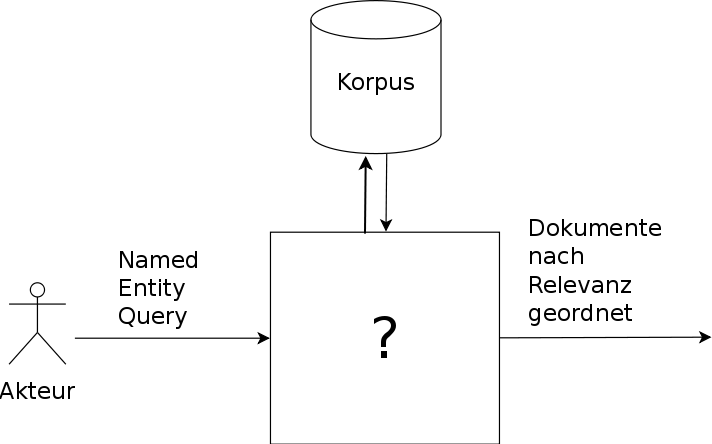
\includegraphics[scale=.2]{pics/overview}
	\end{tabular}
	\caption{Häufige Suchanfrage an Suchmaschinen}
	\label{tab:freq_query}
\end{table}\\
Ein Problem bei solchen Suchanfragen ist es, die Häufigkeit der \textbf{named entity} in Dokumenten richtig zu erfassen\cite{paper:Na}.
Denn die Referenzierung des Objektes, das sich hinter einem Eigennamen verbirgt, wird sowohl mit dem Eigennamen selbst, als auch mit kompakteren Ausdrücken vorgenommen.\\
So wird beispielsweise in einem Text, der von Peter Chen handelt, die Person \textit{Peter Chen} auch mit \textit{"`er"'} referenziert.\\
\\
\fbox{ 
\begin{minipage}{12cm}
	"`\textbf{Chen} has recieved serveral awards in the fields of Information Technology. \textbf{He} received the Data Resource Management Technology Award [\ldots]"' \cite{wiki:peter_chen}
\end{minipage}
}\\
\\
In der folgenden Hausarbeit wird ein statistisches Verfahren erklärt, welches die Häufigkeit von Eigennamen in Dokumenten schätzen soll. Grundlage für diese Ausarbeitung ist ein Paper der Herren Na und Ng über "`A 2-Poisson Model for Probabilistic Coreference of Named Entities for Improved Text Retrieval"'\cite{paper:Na}.

% References (Literaturverzeichnis):
% a) Style (with abbreviations: use alpha):
\bibliographystyle{plainnat-d}
% b) The File:
\newpage
\bibliography{seminararbeit}

\end{document}
